\documentclass{controle}
\usepackage{main}

\printanswers{}

\title{Controle n°4 (Session 2) : Probabilités, vecteurs}
\author{Seconde 3}
\date{}

\begin{document}
\titleandname{}
\instructions{}
\begin{questions}
\titledquestion{Question de cours}[3]
\begin{parts}
\part[1] Soit $\vect{u}$ et $\vect{v}$ deux vecteurs colinéaires. A-t-on forcément $\vect{u} = \vect{v}$ ?
\part[1] Soient deux points du plan $A$ et $B$, et $I$ le milieu du segment $[AB]$. Que peut-on dire des vecteurs $\vect{AI}$ et $\vect{IB}$ ?
\part[1] Les points $M$, $N$ et $P$ sont alignés. Que peut-on dire des vecteurs $\vect{MN}$ et $\vect{MP}$ ?
\end{parts}

\begin{solution}[0.5cm]
\begin{parts}
\part Non, colinéarité ne veut pas dire égalité.
\part On a $\vect{AI} = \vect{IB}$.
\part Les vecteurs $\vect{MN}$ et $\vect{MP}$ sont colinéaires. 
\end{parts}
\end{solution}

\titledquestion{Vecteurs et translations}[5]
Sur la figure suivante, les triangles représentés sont tous équilatéraux.
\begin{center}
\begin{tikzpicture}[scale=2]
\coordinate (A) at (0,0);
\coordinate (B) at ($(A) + (0:1)$); 
\coordinate (C) at ($(A) + (60:1)$);
\coordinate (D) at ($(B) + (0:1)$);
\coordinate (E) at ($(B) + (60:1)$);
\coordinate (F) at ($(D) + (0:1)$);
\coordinate (G) at ($(D) + (60:1)$);
\coordinate (I) at ($(C) + (60:1)$);
\coordinate (K) at ($(E) + (60:1)$);
\coordinate (M) at ($(I) + (60:1)$);

\draw (A) -- (B) -- (C) -- cycle;
\draw (B) -- (D) -- (E) -- cycle;
\draw (D) -- (F) -- (G) -- cycle;
\draw (C) -- (E) -- (I) -- cycle;
\draw (E) -- (G) -- (K) -- cycle;
\draw (I) -- (K) -- (M) -- cycle;

\draw (A) node[below left] {$A$};
\draw (B) node[below] {$B$};
\draw (C) node[left] {$C$};
\draw (D) node[below] {$D$};
\draw (E) node[below] {$E$};
\draw (F) node[below right] {$F$};
\draw (G) node[right] {$G$};
\draw (I) node[left] {$I$};
\draw (K) node[right] {$K$};
\draw (M) node[above] {$M$};
\end{tikzpicture}
\end{center}

Dans cet exercice, on ne demande aucune justification. Pour chaque point d'origine $O$ donné et chaque vecteur $\vect{u}$ donné, donner l'image de $O$ par le vecteur $\vect{u}$. Par exemple, si $O = A$ et $\vect{u} = \vect{IK}$, alors on obtient $B$.
\begin{parts}
\begin{minipage}{0.45\textwidth}
\part $O = E$ et $\vect{u} = \vect{EG}$ :
\part $O = I$ et $\vect{u} = \vect{GD}$ :
\part $O = D$ et $\vect{u} = \vect{KM}$ :
\part $O = M$ et $\vect{u} = \vect{EB}$ :
\part $O = F$ et $\vect{u} = -\vect{CE}$ :
\end{minipage}
\hfill
\begin{minipage}{0.45\textwidth}
\part $O = G$ et $\vect{u} = \vect{GE} + \vect{EI}$ :
\part $O = G$ et $\vect{u} = \vect{KI} + \vect{IE}$ :
\part $O = D$ et $\vect{u} = 2\vect{EC}$ :
\part $O = M$ et $\vect{u} = -2\vect{EK}$ :
\part $O = K$ et $\vect{u} = \vect{CA} - \vect{EI}$ :
\end{minipage}
\end{parts}

\begin{solution}[0.5cm]
\begin{parts}
\begin{minipage}{0.45\textwidth}
\part $G$
\part $C$
\part $E$
\part $I$
\part $D$
\end{minipage}
\hfill
\begin{minipage}{0.45\textwidth}
\part $I$
\part $D$
\part $A$
\part $C$
\part $D$
\end{minipage}
\end{parts}
\end{solution}



\titledquestion{Vecteurs et parallélogrammes}[7]:
\begin{parts}
\part[0,5] Soient quatre points $A, B, C, D$ tels que $\vect{AB} = \vect{DC}$. Quelle est la nature du quadrilatère $ABCD$ ?
\part[1] Soit $R$, $S$ et $T$ trois points du plan représenté ci-dessous :
\begin{center}
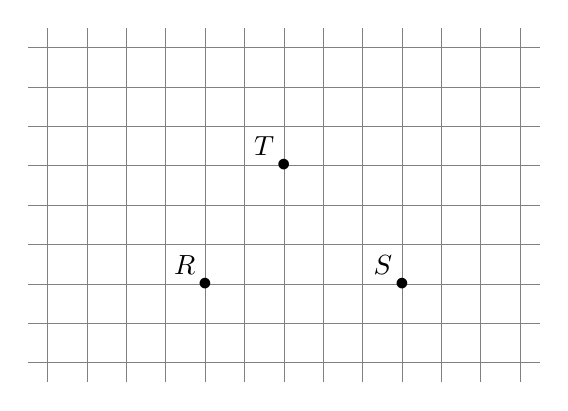
\begin{tikzpicture}
\draw[help lines] (-0.25,-0.25) grid[step=0.5] (6.25,4.25);

\draw (2,1) node {$\bullet$} node[above left] {$R$};
\draw (4.5,1) node {$\bullet$} node[above left] {$S$};
\draw (3,2.5) node {$\bullet$} node[above left] {$T$};
\end{tikzpicture}
\end{center}
Placer le point $E$ tel que $\vect{TE} = \vect{RT}$.
\part[1] Placer le point $P$ tel que $\vect{RP} = \vect{RS} + \vect{RT}$.
\part[1,5] Montrer que $\vect{TP} = \vect{RS}$. Pour cela, on pourra utiliser la relation de Chasles suivante :
\begin{equation*}
\vect{TP} = \vect{TR} + \vect{RP}
\end{equation*}
\part[1] Placer le point $U$ tel que $\vect{SU} = \vect{SR} + \vect{ST}$.
\part[1,5] Montrer que $\vect{RU} = \vect{ST}$. On utilisera une relation de Chasles bien choisie sur le vecteur $\vect{RU}$.
\part[0,5] Quelle est la nature des quadrilatères $SRUT$ et $RSPT$ ? Justifier à l'aide des questions précédentes.
\end{parts}

\begin{solution}[0.5cm]
\begin{center}
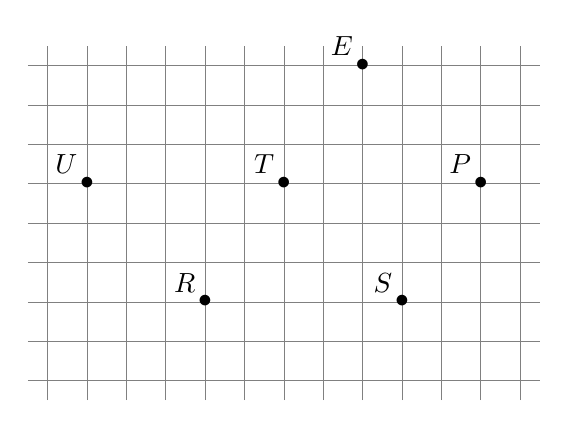
\begin{tikzpicture}
\draw[help lines] (-0.25,-0.25) grid[step=0.5] (6.25,4.25);

\draw (2,1) node {$\bullet$} node[above left] {$R$};
\draw (4.5,1) node {$\bullet$} node[above left] {$S$};
\draw (3,2.5) node {$\bullet$} node[above left] {$T$};
\draw (4,4) node {$\bullet$} node[above left] {$E$};
\draw (5.5,2.5) node {$\bullet$} node[above left] {$P$};
\draw (0.5,2.5) node {$\bullet$} node[above left] {$U$};
\end{tikzpicture}
\end{center}
\begin{parts}
\part Le quadrilatère $ABCD$ est un parallélogramme.
\part Voir figure au début du corrigé.
\part Voir figure au début du corrigé.
\part \hfill 
\begin{equation*}
\begin{aligned}
\vect{TP} = \vect{TR} + \vect{RP} &= \vect{TR} + \vect{RS} + \vect{RT}\\
&= \vect{TR} + \vect{RT} + \vect{RS}\\
&= \vect{TT} + \vect{RS}\\
&= \vect{0} + \vect{RS} = \vect{RS}\\
\end{aligned}
\end{equation*}
\part Voir figure au début du corrigé.
\part \hfill 
\begin{equation*}
\begin{aligned}
\vect{RU} = \vect{RS} + \vect{SU} &= \vect{RS} + \vect{SR} + \vect{ST}\\
&= \vect{RR} + \vect{ST}\\
&= \vect{0} + \vect{ST}\\
&= \vect{ST}
\end{aligned}
\end{equation*}
\part On en déduit que ces deux quadrilatères sont des parallélogrammes. En effet, car $\vect{RU} = \vect{ST}$ et $\vect{TP} = \vect{RS}$.
\end{parts}
\end{solution}





\titledquestion{Vecteurs et algèbre}[5]
\begin{parts}
\part[0,5] Rappeler la relation de Chasles en recopiant et complétant l'égalité suivante :
\begin{equation*}
\vect{A\dots} + \vect{B\dots} = \vect{AC}
\end{equation*}
\part[0,5] Simplifier $- \vect{AB}$.
\part À partir des égalités suivantes, trouver $k$ tel que $\vect{AB} = k\vect{AC}$.
\begin{subparts}
\subpart[0,5] $\vect{AB} = \vect{CA}$
\subpart[0,5] $\vect{AB} = 7\vect{AC} + 3\vect{CA}$
\subpart[1] $\vect{AB} + \vect{AC} = 2\vect{AB} - 5\vect{AC}$
\subpart [1] $\vect{AB} + \vect{AC} = 3\vect{BC}$ (Indication : on utilisera $\vect{BC} = \vect{BA} + \vect{AC}$)
\subpart [1] $3\vect{CB} = 2\vect{AB}$ (Indication : on utilisera $\vect{CB} = \vect{CA} + \vect{AB}$)
\end{subparts}
\end{parts}
\begin{solution}
\begin{parts}
\part $\vect{AB} + \vect{BC} = \vect{AC}$.
\part Les vecteurs $\vect{u}$ et $\vect{v}$ ont la même direction : on dit qu'ils sont colinéaires.
\part
\begin{subparts}
\subpart $\vect{AB} = \vect{CA} = - \vect{AC}$, donc $k = -1$.
\subpart $\vect{AB} = 7\vect{AC}+ 3\vect{CA} = 7\vect{AC} - 3\vect{AC} = 4\vect{AC}$, donc $k = 4$.
\subpart
\begin{equation*}
\begin{aligned}
&\vect{AB} + \vect{AC} = 2\vect{AB} - 5\vect{AC}\\
\Leftrightarrow& \vect{AB} - 2\vect{AB} = -5\vect{AC} - \vect{AC}\text{ (On regroupe les termes)}\\
\Leftrightarrow& -\vect{AB} = -6\vect{AC} \text{ (On réduit)}\\
\Leftrightarrow& \vect{AB} = 6\vect{AC}\text{ (On divise par $-1$ des deux côtés)}\\
\end{aligned}
\end{equation*}
Donc $k = 6$
\subpart
\begin{equation*}
\begin{aligned}
&\vect{AB} + \vect{AC} = 3\vect{BC}\\
\Leftrightarrow&\vect{AB} + \vect{AC} = 3(\vect{BA} + \vect{AC}) \text{ (On utilise l'indication)}\\
\Leftrightarrow&\vect{AB} + \vect{AC} = 3\vect{BA} + 3\vect{AC} \text{ (On développe)}\\
\Leftrightarrow&\vect{AB} - 3\vect{BA} = 3\vect{AC} - \vect{AC}\text{ (On regroupe les termes)}\\
\Leftrightarrow&\vect{AB} + 3\vect{AB} = 3\vect{AC} - \vect{AC}\text{ (Car $\vect{BA} = - \vect{AB}$)}\\
\Leftrightarrow&4\vect{AB} = 2\vect{AC}\text{ (On réduit)}\\
\Leftrightarrow&\vect{AB}=\dfrac{1}{2}\vect{AC}\text{ (On divise par $4$)}
\end{aligned}
\end{equation*}
Donc $k = \dfrac{1}{2}$
\subpart
\begin{equation*}
\begin{aligned}
&3\vect{CB}=2\vect{AB}\\
\Leftrightarrow&3(\vect{CA} + \vect{AB})=2\vect{AB}\text{ (On utilise l'indication)}\\
\Leftrightarrow&3\vect{CA} + 3\vect{AB}=2\vect{AB}\text{ (On développe)}\\
\Leftrightarrow&3\vect{CA}=2\vect{AB} - 3\vect{AB}\text{ (On regroupe les termes)}\\
\Leftrightarrow&-3\vect{AC}=2\vect{AB} - 3\vect{AB}\text{ (On utilise $\vect{CA} = -\vect{AC}$)}\\
\Leftrightarrow&-3\vect{AC}=-\vect{AB}\text{ (On réduit)}\\
\Leftrightarrow&3\vect{AC}=\vect{AB}\text{ (On divise par $-1$)}\\
\end{aligned}
\end{equation*}
Donc $k = 3$.
\end{subparts}
\end{parts}
\end{solution}




% \titledquestion{Vecteurs et Modélisation}[5]
% Soit $ABC$ un triangle quelconque. Soient $D$ et $E$ deux points tels que $\vect{AD} = \dfrac{1}{4}\vect{AB}$ et $\vect{AE}=4\vect{AC}$
% \begin{parts}
% \part[1] Construire le triangle $ABC$ ainsi que le points $D$ et $E$.
% \part[1] En utilisant l'égalité $\vect{DC} = \vect{DA} + \vect{AC}$, montrer que
% \begin{equation*}
% \vect{DC} = \vect{AC} - \dfrac{1}{4}\vect{AB}
% \end{equation*}
% \part[1] En utilisant l'égalité $\vect{BE} = \vect{BA} + \vect{AE}$, montrer que
% \begin{equation*}
% \vect{BE} = 4\vect{AC} - \vect{AB}
% \end{equation*}
% \part[1] Déduire des questions précédentes que $\vect{BE} = 4\vect{DC}$.
% \part[1] En déduire la nature du quadrilatère $BECD$.
% \end{parts}
% \begin{solution}
% \begin{parts}
% \part
% \part On part de l'égalité $\vect{DC} = \vect{DA} + \vect{AC}$. Alors,
% \begin{equation*}
% \begin{aligned}
% \vect{DC} &= \vect{DA} + \vect{AC}\\ 
% &= -\vect{AD} + \vect{AC}\\
% &= -(\dfrac{1}{4}\vect{AB}) + \vect{AC}\\
% &= \vect{AC} - \dfrac{1}{4}\vect{AB}
% \end{aligned}
% \end{equation*}
% \part On part de l'égalité $\vect{BE} = \vect{BA} + \vect{AE}$. Alors,
% \begin{equation*}
% \begin{aligned}
% \vect{BE} &= \vect{BA} + \vect{AE}\\ 
% &= \vect{BA} + (4\vect{AC})\\
% &= -\vect{AB} + (4\vect{AC})\\
% &= 4\vect{AC} - \vect{AB}
% \end{aligned}
% \end{equation*}
% \part On part de $4\vect{DC}$ pour montrer l'égalité de l'énoncé.
% \begin{equation*}
% \begin{aligned}
% 4\vect{DC} &= 4(\vect{AC} -\dfrac{1}{4}\vect{AB})\\
% &= 4\vect{AC} - 4 \times \dfrac{1}{4} \vect{AB}\\
% &= 4\vect{AC} - \vect{AB}\\
% &= \vect{BE}
% \end{aligned}
% \end{equation*}
% Ainsi, $\vect{BE} = 4\vect{DC}$.
% \part Le quadrilatère $BECD$ est un trapèze.
% \end{parts}

% \end{solution}
\end{questions}
\end{document}